\documentclass[conference]{IEEEtran}
\IEEEoverridecommandlockouts
% The preceding line is only needed to identify funding in the first footnote. If that is unneeded, please comment it out.
\usepackage{cite}
\usepackage{amsmath,amssymb,amsfonts}
\usepackage{algorithmic}
\usepackage{graphicx}
\usepackage{textcomp}
\usepackage{xcolor}
\usepackage{float} 
\def\BibTeX{{\rm B\kern-.05em{\sc i\kern-.025em b}\kern-.08em
    T\kern-.1667em\lower.7ex\hbox{E}\kern-.125emX}}
\begin{document}

\title{Detección de riesgos cardíacos en deportistas\\
}

\author{
\IEEEauthorblockN{Yanko Acuña Villaseca}
\IEEEauthorblockA{\textit{Departamento de Ciencias de la Computación} \\
\textit{Facultad de Ingeniería} \\
\textit{Universidad de Talca}\\
Talca, Chile \\
yacuna20@alumnos.utalca.cl}
\and 
\IEEEauthorblockN{César Astudillo}
\IEEEauthorblockA{\textit{Departamento de Ciencias de la Computación} \\
\textit{Facultad de Ingeniería} \\
\textit{Universidad de Talca}\\
Talca, Chile \\
yacuna20@alumnos.utalca.cl}
}

\maketitle

\begin{abstract}
Se busca predecir el diagnóstico general de un ECG de un deportista, 
identificando si es normal o de riesgo, aplicando inteligencia artificial.
Para esto se entrena un modelo con la base de datos "Lobachevsky University Electrocardiography Database", 
y se prueba con la base de datos "Norwegian Endurance Athlete ECG Database".
Esto con un enfoque en la detección de riesgos cardíacos en deportistas, 
buscando prevenir la muerte súbita cardíaca en deportistas de alto rendimiento.

\end{abstract}

\begin{IEEEkeywords}
diagnóstico de ECG, detección de riesgos cardíacos en deportistas, Muerte súbita cardiaca, 
medicina deportiva, inteligencia artificial aplicada a la medicina.
\end{IEEEkeywords}

\section{Introducción}
La muerte súbita cardíaca es un peligro presente en los deportes de alto rendimiento, los deportistas
 se enfrentan a grandes esfuerzos en donde el cuerpo humano es llevado al límite. El corazón de un atleta
  de alto rendimiento está adaptado a sostener esfuerzos altos durante un tiempo más prolongado, estos 
  cambios en el corazón no representan un peligro para el atleta, sin embargo, con la aparición de estos 
  nuevos cambios, el corazón de atleta puede camuflar una miocardiopatía.

  Se busca predecir el diagnóstico general de un ECG de un deportista, identificando si es normal o de riesgo,
  para esto se utiliza inteligencia artificial para entrenar un modelo que permita clasificar los ECGs de los
    deportistas. En este caso se entrena un modelo con la base de datos "Lobachevsky University Electrocardiography Database",
    y se prueba con la base de datos "Norwegian Endurance Athlete ECG Database", 
    ambas bases de datos son extraídas de PhysioNet. 


    

\section{Descripción del problema}

Los deportistas de alto rendimiento generan adaptaciones en el corazón, derivando en un corazón de atleta. 
Estas adaptaciones pueden ser factores de riesgo para personas no deportistas, por lo que es importante 
detectar estas anomalías y evaluar si corresponde a un riesgo para el deportista. Debido a que un mal 
diagnóstico puede derivar en una muerte cardíaca súbita.

Para solucionar este problema se plantea un modelo que busca predecir el diagnóstico general de un ECG
 de un deportista, se espera que \textbf{el modelo clasifique si se tiene un ECG normal o de riesgo}. 
 Para así, alertar un posible riesgo y requerir la interpretación de un cardiólogo.


\section{Descripción de los datos}
Se tiene la base de datos "Norwegian Endurance Athlete ECG Database" \cite{b1} que contiene 28 
ECG de 12 derivaciones de atletas de alto rendimiento de Noruega. Debido a la baja cantidad de 
datos se optó por expandir la cantidad de datos, para esto se usó “Lobachevsky University 
Electrocardiography Database” \cite{b2}. Esta base de datos contiene 200 ECG de 12 derivaciones 
de personas que no son necesariamente deportistas, para utilizar estos datos en un contexto de 
detectar anomalías en deportistas, solo se considera los datos de los pacientes hasta 45 años, 
por lo que finalmente se tienen 69 pacientes de la nueva base de datos.

Las bases de datos tienen diferencias entre el formato de presentación del diagnóstico, pero en 
ambos casos \textbf{el diagnóstico es realizado por cardiólogos}, en el caso de la BD de Atletas 
Noruegos el cardiólogo es especializado en medicina deportiva, además, se tiene adicionalmente un 
diagnóstico del algoritmo Marquette SL12. En la BD de deportistas, las etiquetas se presentan en 
un listado, donde primero se indica el tipo de ritmo, posterior a esto se agregan si es que existen 
anomalías cardíacas, y finalmente se indica el diagnóstico general del ECG, si es normal, limítrofe 
o anormal. En el caso de la BD de Lobachevsky University, se indica el tipo de ritmo cardíaco, el eje 
eléctrico del corazón y se agregan si es que existen anomalías, en este caso no indica el diagnóstico general del ECG.

Para normalizar y estandarizar los datos de ambos ECG se hizo se normaliza los datos de los ECG 
ajustando los valores a un rango de 0 a 1 y luego ajusta la frecuencia de muestreo del ECG a 500 Hz. 
Si la frecuencia de muestreo original no es 500 Hz, realiza una interpolación para cambiar la frecuencia.
\begin{figure}[H]
    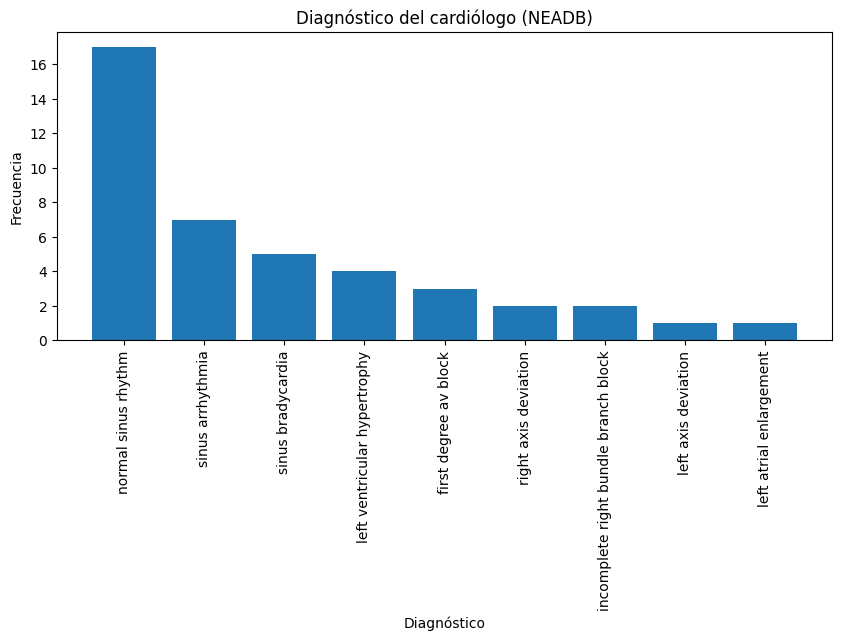
\includegraphics[width=0.5\textwidth]{./graficos/hallazgosNEADB.png}
    \caption{Hallazgos NEADB}
    \label{fig}
\end{figure}
\begin{figure}[H]
    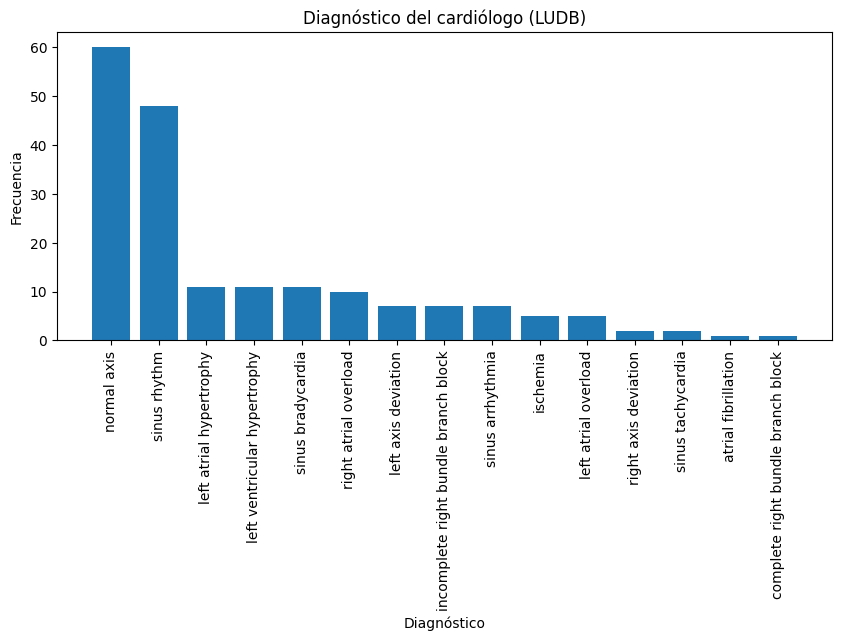
\includegraphics[width=0.5\textwidth]{./graficos/hallazgosLUDB.png} 
    \caption{Hallazgos LUDB}
    \label{fig}
\end{figure}

\section{Generación de diagnósticos de la nueva base de datos}
Debido a que falta el diagnóstico general de cada ECG de la BD de Lobachevsky University, 
se evaluaron las etiquetas de los hallazgos en base al “Consenso Internacional de los Criterios 
para la Interpretación del ECG en Atletas” \cite{b3}. Estos criterios buscan disminuir los falsos 
positivos mejorando la detección de anomalías que pueden derivar en una muerte cardíaca súbita.

Los hallazgos se clasifican según el riesgo que presenta una de estas anomalías hacia los deportistas. 
Para los datos de Lobachevsky University, se tomó en cuenta las etiquetas presentes, en donde se clasificó 
como de riesgo una desviación del eje eléctrico del corazón, crecimiento en el auricular derecho o izquierdo 
y un bloqueo completo de la rama derecha o algún tipo de isquemia.

A continuación, se presentan las tablas que clasifica los hallazgos en habituales, borderline y anormales del 
"Consenso Internacional de los Criterios para la Interpretación del ECG en Atletas"

\begin{table}[H]
    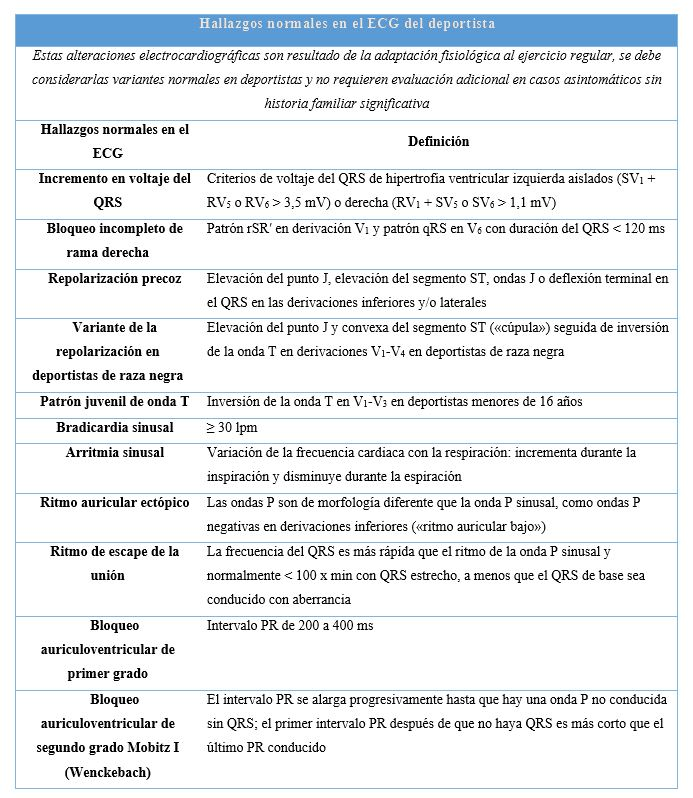
\includegraphics[width=0.5\textwidth]{./graficos/Tabla1HallazgosHabituales.jpg}
    \caption{Hallazgos Habituales}
\end{table}

\begin{table}[H]
    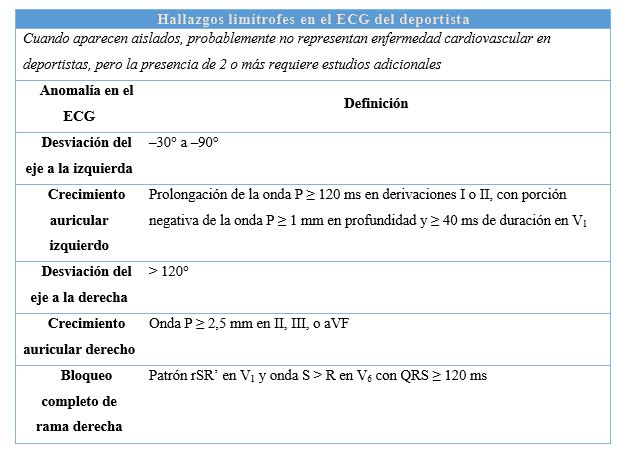
\includegraphics[width=0.5\textwidth]{./graficos/Tabla2HallazgosBorderline.jpg}
    \caption{Hallazgos Borderline}
\end{table}

\begin{table}[H]
    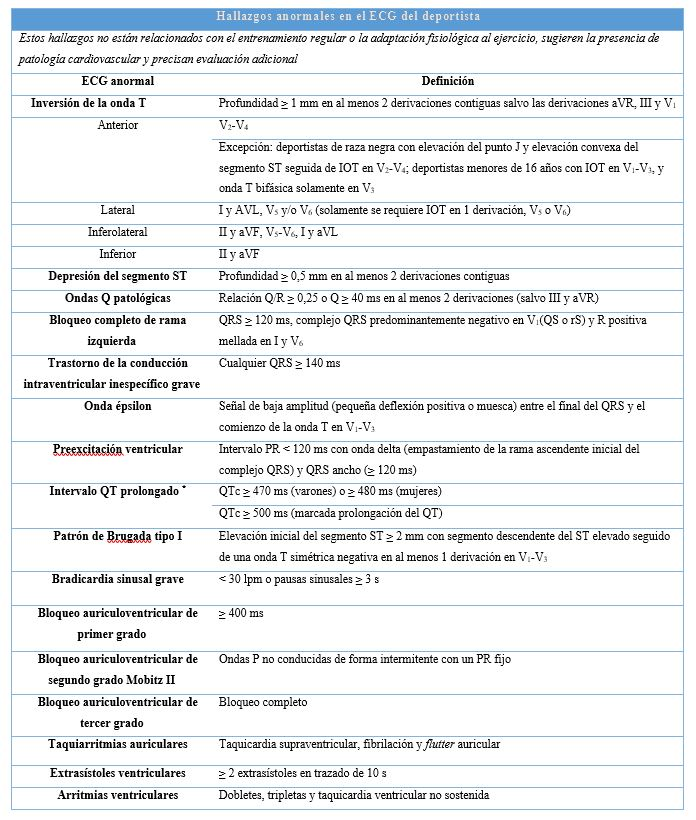
\includegraphics[width=0.5\textwidth]{./graficos/Tabla3HallazgosAnormales.jpg}
    \caption{Hallazgos Anormales}
\end{table}



\section{Gráficos de diagnósticos de los ECG }

Se presentan los diagnósticos generales de los ECG de ambas bases de datos.

\begin{figure}[H]
    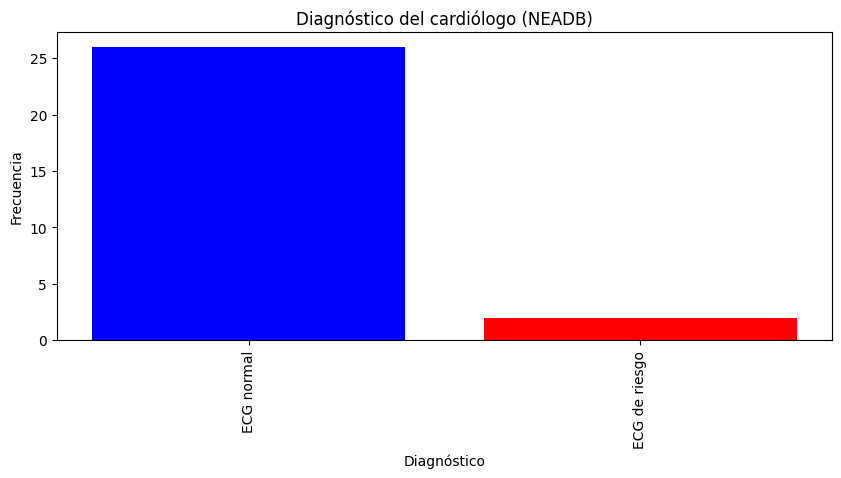
\includegraphics[width=0.5\textwidth]{./graficos/diagnosticoGeneralNEADB.png}
    \caption{Diagnóstico general de NEADB}
\end{figure}

\begin{figure}[H]
    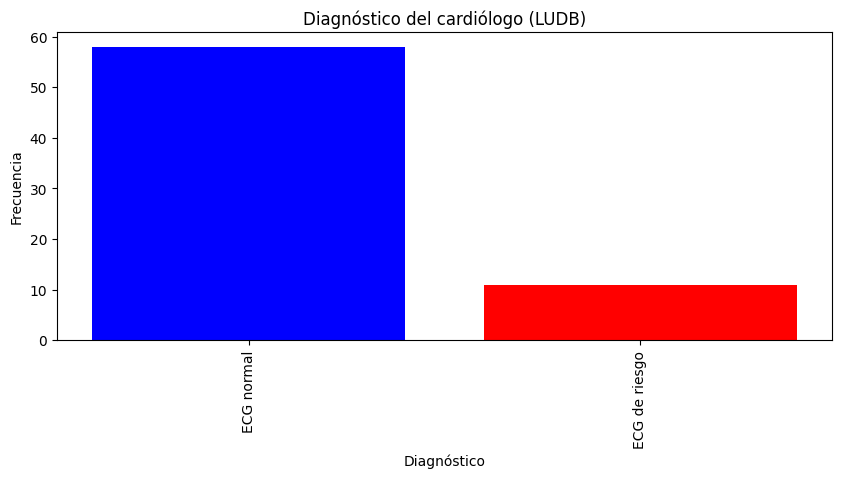
\includegraphics[width=0.5\textwidth]{./graficos/diagnosticoGeneraLUDB.png}
    \caption{Diagnóstico general de LUDB}
\end{figure}

\section{Gráfico PCA para visualizar ECG normales y de riesgo}

Aunque no se puede diagnosticar si un ECG es de riesgo mediante este gráfico, si se logra visualizar 
un sesgo entre la posición de los ECG y la clasificación, debido a que hacia los bordes se encuentran
 los casos que se clasifican como de riesgo, y existe una zona en donde se agrupa la mayor cantidad de
  casos normales. Debido a que existe una diferencia de distancia entre el grupo de ECGs normales y los
   casos de bordes, se podría calcular la distancia de un ECG frente a los datos de entrenamiento y buscar 
   los casos más cercanos, para así detectar los casos de riesgo.

\begin{figure}[H]
    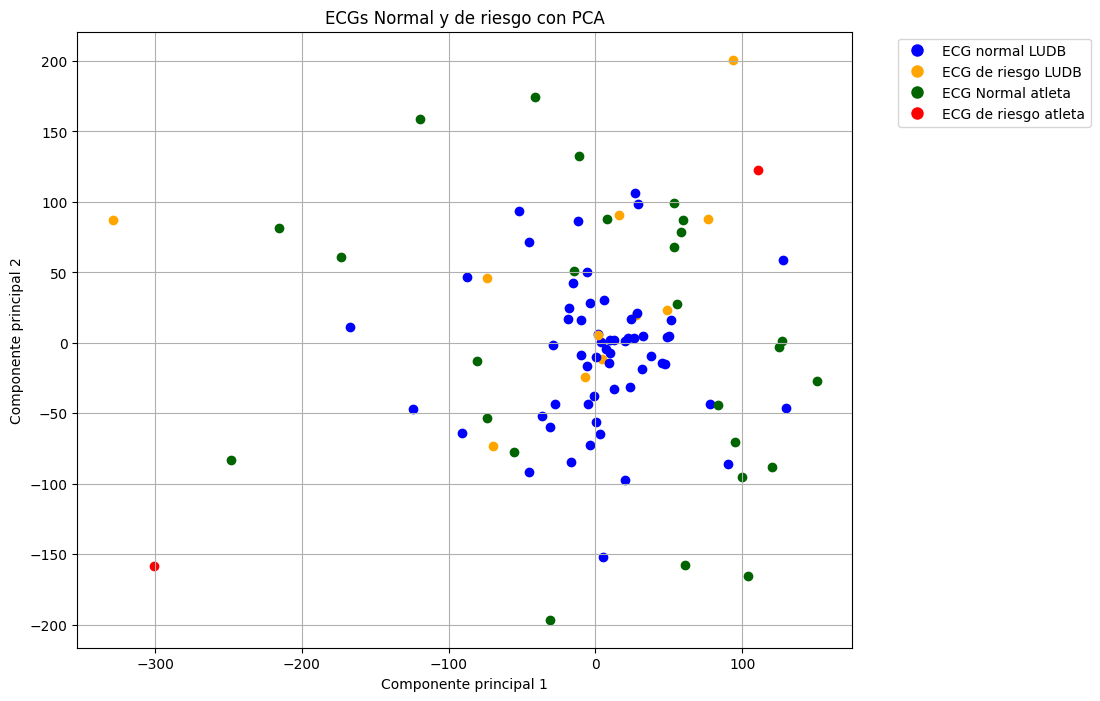
\includegraphics[width=0.5\textwidth]{./graficos/graficoPCA.png}
    \caption{Gráfico PCA}
\end{figure}

\section{Uso de los datos}
Para este problema se utilizarán los datos de la BD de Lobachevsky University para entrenar el modelo,
 utilizando las etiquetas generadas para los diagnósticos, y se utilizará la BD de Atletas Noruegos para
  probar el modelo entrenado. 

\section{Comparación de métricas de diferentes modelos de clasificación}
Con el fin de usar un modelo de clasificación que se adapte a las necesidades del problema, 
se entrenaron diferentes modelos y se calcularon las métricas obtenidas al realizar predicciones. 
Los modelos entrenados fueron los siguientes: K-nearest neighbors con Dynamic Time Warping (DTW), 
Decision Tree, Naive Bayes, Support vector machine (SVM) y XGBoost.

Los modelos como Decision Tree, Naive Bayes, Support vector machine (SVM) y XGBoost, fueron 
entrenados con los datos estadísticos de cada señal ECG.

Las métricas de exactitud, precisión, recall y f1 son las siguientes:

\begin{figure}[H]
    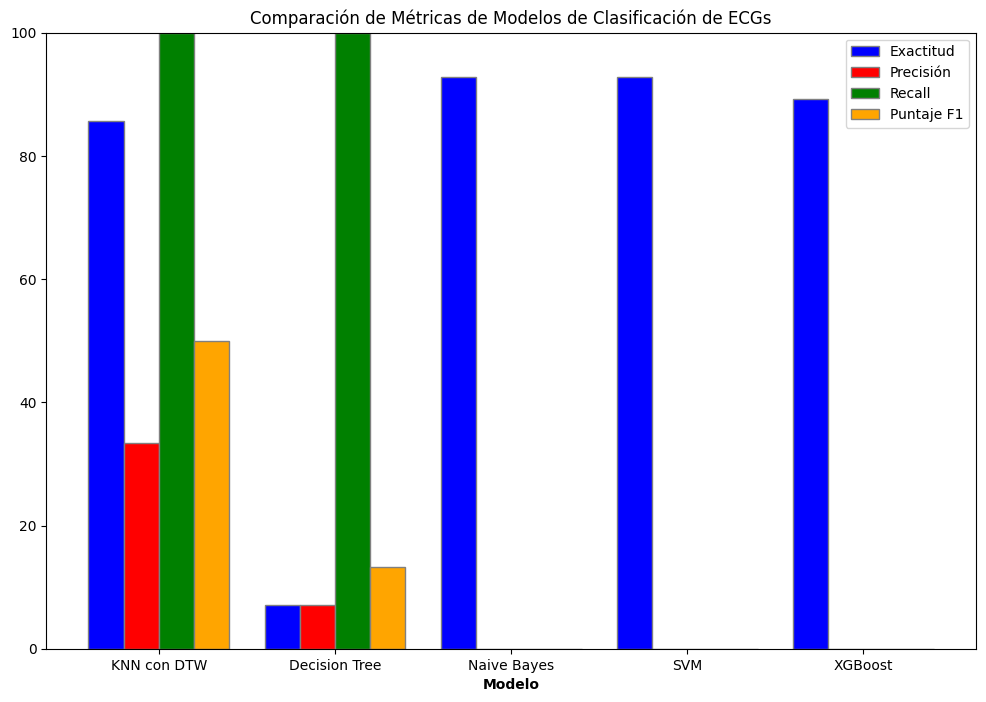
\includegraphics[width=0.5\textwidth]{./graficos/comparacionModelosClasificacion.png}
    \caption{Gráfico de comparación entre modelos}
\end{figure}

Para este caso es importante tener el mayor porcentaje de recall debido a que se deben detectar 
todos los casos de riesgo. Según las métricas, es posible utilizar los modelos de KNN con DTW y 
XGBoost. El problema de XGBoost es que, aunque no genera demasiados falsos positivos, este no 
clasifica correctamente los casos de riesgo.

\section{Selección y Justificación de Modelos}
Para predecir el diagnóstico general de un ECG, identificando si es \textbf{normal, o de riesgo}, se
 utilizó el modelo de \textbf{K-nearest neighbors (KNN)} utilizando \textbf{Dynamic Time Warping (DTW)}
  como métrica de distancia, para así, comparar los ECGs y encontrar el más cercano. 
Se utilizó esta técnica debido a la baja cantidad de datos, lo que dificultaba aplicar técnicas
 que requieren un mayor volumen de datos como Random Forest o algún algoritmo de aprendizaje supervisado.

Una de las principales ventajas de utilizar DTW en el análisis de ECGs, es su capacidad para alinear 
y comparar señales de diferentes longitudes o con variaciones en el tiempo. Para el caso de los ECGs,
 esto es útil debido a las siguientes razones:

\subsection{Manejo de Variabilidad Temporal}
Los ECGs suelen tener variaciones en la frecuencia y duración de los latidos cardíacos. DTW permite 
alinear estas señales, ignorando las pequeñas diferencias temporales, permitiendo detectar patrones
 de una mejor manera.

\subsection{Eficiencia con Pocos Datos}
Al no requerir grandes volúmenes de datos para entrenamiento, DTW se adapta de manera ideal para
 conjuntos de datos pequeños y permite encontrar patrones relevantes.

Este modelo es relevante debido a que permite comparar las señales de ondas sin que afecten los 
pequeños desfases de tiempos, además al comparar señales permite comparar entre las formas de las ondas, 
detectando con precisión las similitudes entre las señales. 

Además, al implementar diferentes modelos, se obtuvo que el modelo KNN con DTW presenta mejores 
métricas al realizar predicciones.

\section{Implementación y Evaluación de Modelos}
El modelo de K-nearest neighbors (KNN) con Dynamic Time Warping (DTW) como métrica de distancia
 es entrenado con la BD de Lobachevsky University, y para probar la precisión del modelo se 
 utiliza la BD de Atletas Noruegos.
La implementación de KNN con DTW consiste en que, para cada ECG de la BD de Atletas Noruegos,
 se calcula las distancias DTW con respecto a cada ECG del conjunto de entrenamiento.
  Con las distancias calculadas con respecto a todos los ECGs de entrenamiento, se buscan los
   k vecinos más cercanos, y el diagnóstico del ECG corresponde al grupo mayoritario de los vecinos hallados.

\section{Evaluación de variantes de KNN}
Para obtener mejores resultados se optó por modificar el algoritmo KNN, en este caso se 
implementó que en base a los n vecinos hallados, si alguno de estos vecinos corresponde 
a un ECG de riesgo, el ECG evaluado se clasifica como de riesgo.
Se evaluaron los resultados de KNN con k igual a 3, 5 y 7, y con el algoritmo del grupo mayor 
y la variante de un vecino de riesgo.

\begin{figure}[H]
    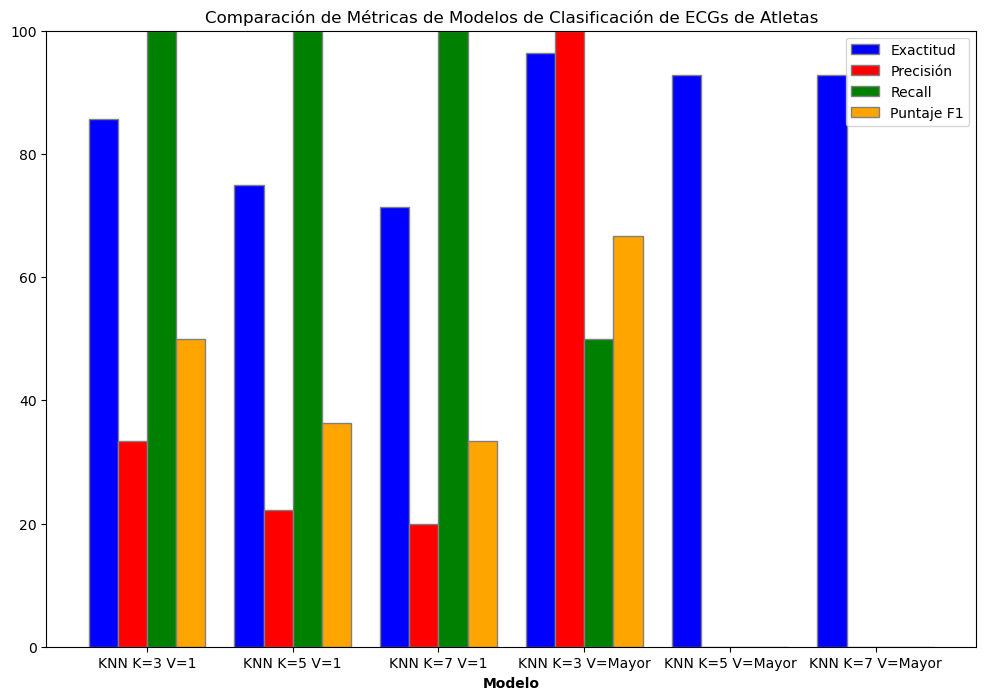
\includegraphics[width=0.5\textwidth]{./graficos/comparacionKNN.png}
    \caption{Gráfico de comparación entre modelos}
\end{figure}

Según los resultados obtenidos, se obtuvo un recall en todas las pruebas realizadas 
con la variante de KNN de tener un vecino de riesgo. La versión estándar de KNN con k igual a 3, 
obtuvo un 100\% de precisión pero no logró clasificar correctamente los casos de riesgo, lo cual, 
en este caso es primordial. Se optó por utilizar k igual a 3 y la versión de tener un vecino de riesgo,
 debido a que al aumentar el valor de k aumenta la aparición de falsos positivos.

Al evaluar el modelo, este entrega una exactitud del 85,71\%, esto debido a que el modelo 
detecta los casos que son de riesgo, pero indica algunos falsos positivos, clasificando casos
 que son normales como de riesgos. Sin embargo, es importante que los casos de riesgo no sean 
 detectados como normales.

\subsection{Matriz de Confusión de Diagnósticos de ECGs de Atletas}
\begin{figure}[H]
    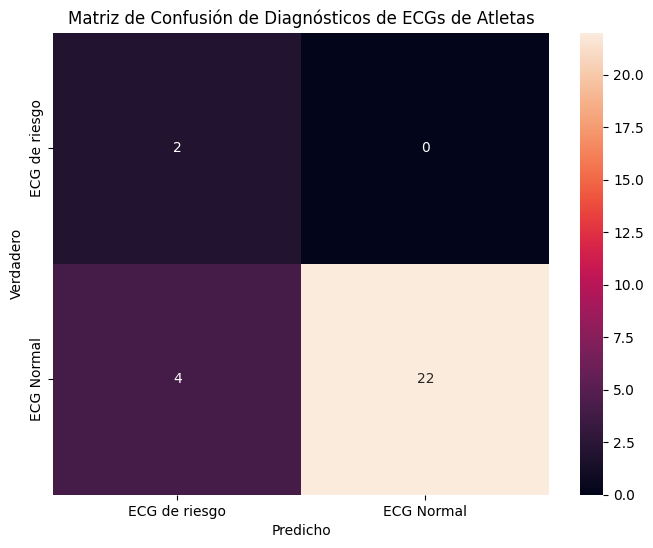
\includegraphics[width=0.5\textwidth]{./graficos/matrizConfusionAtletas.png}
    \caption{Matriz de Confusión Atletas}
\end{figure}

Debido a que en este caso se generan ciertos falsos positivos, se presenta la opción de no
 clasificar este diagnóstico como un completo error, sino que este caso posiblemente sí necesite
  la evaluación de un cardiólogo. Debido a que se posee las etiquetas del algoritmo SL12, 
  se tiene la posibilidad de usar este diagnóstico para comprobar la predicción. 
  Es por esto que cuando el modelo predice un ECG como de riesgo y el cardiólogo no lo 
  contempló de esta manera, se evalúa el diagnóstico del algoritmo SL12. 

Al contemplar este diagnóstico adicional, se obtiene una exactitud del 96,4\%, ya que el 
algoritmo SL12 había clasificado los ECGs que dieron falsos positivos como de riesgo. 
Sin embargo, el cardiólogo al realizar un análisis del paciente descartó los riesgos. 
Por lo que el modelo no se aleja del diagnóstico final, ya que el objetivo del modelo es 
indicar si existe una alerta, para que así un cardiólogo pueda diagnosticar si existe un 
posible riesgo para el deportista.

\subsection{Matriz de Confusión de Diagnósticos de ECGs de Atletas usando etiqueta de SL12}
\begin{figure}[H]
    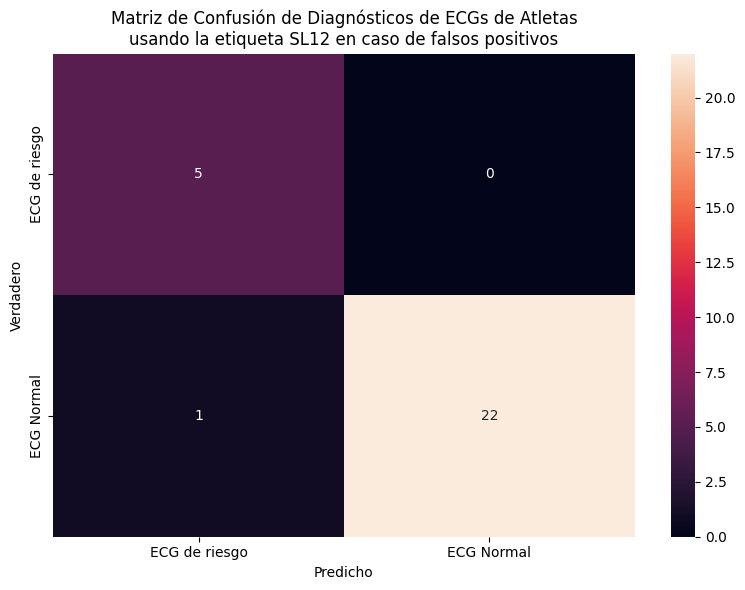
\includegraphics[width=0.5\textwidth]{./graficos/matrizConfusionAtletasSL12.png}
    \caption{Matriz de Confusión Atletas con SL12}
\end{figure}

El recall es de 100\% ya que se detectaron todos los casos de riesgo correctamente, 
lo que es primordial para el modelo. Adicionalmente, se tiene un 33,33\% de precisión, 
ya que se generaron algunos falsos positivos, sin embargo, este porcentaje aumenta a 83.33\% 
si se consideran los diagnósticos del SL12. El F1 tiene un 50\% considerando las etiquetas de
 los cardiólogos y un 90,91\% considerando adicionalmente la etiqueta del SL12.

\subsection{Métricas de la evaluación}
\begin{figure}[H]
    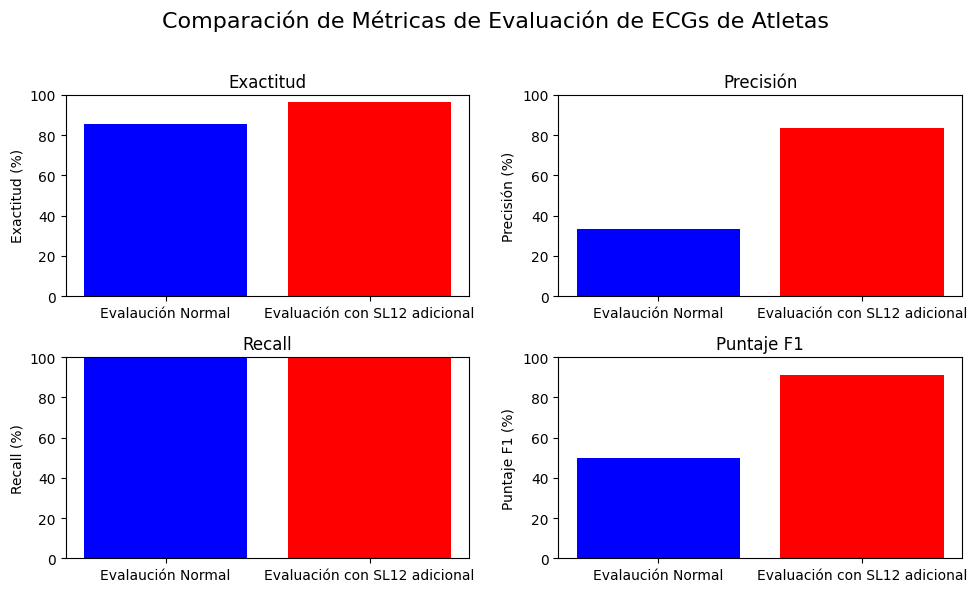
\includegraphics[width=0.5\textwidth]{./graficos/metricasDTW.png}
    \caption{Métricas de la evaluación con DTW}
\end{figure}

\section{Comparación de gráfico PCA con predicciones realizadas}

\subsection{Gráfico de etiquetas de cardiólogos}
\begin{figure}[H]
    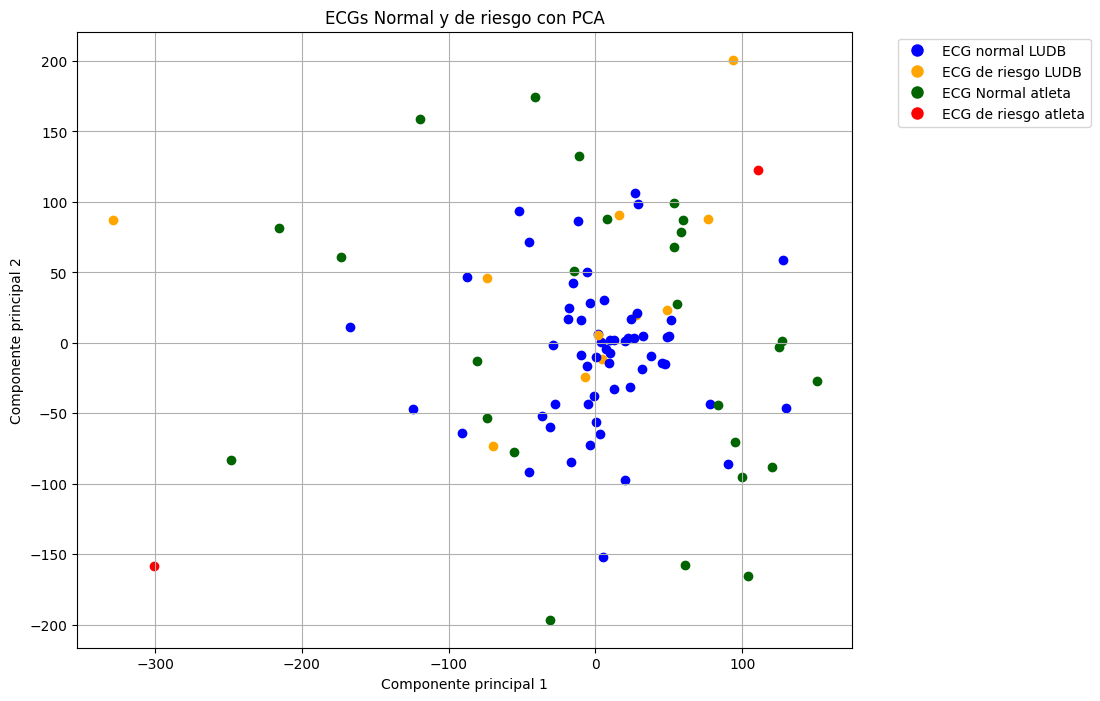
\includegraphics[width=0.5\textwidth]{./graficos/graficoPCA.png}
    \caption{Gráfico PCA}
\end{figure}

\subsection{Gráfico de etiquetas de predichas por el modelo}
\begin{figure}[H]
    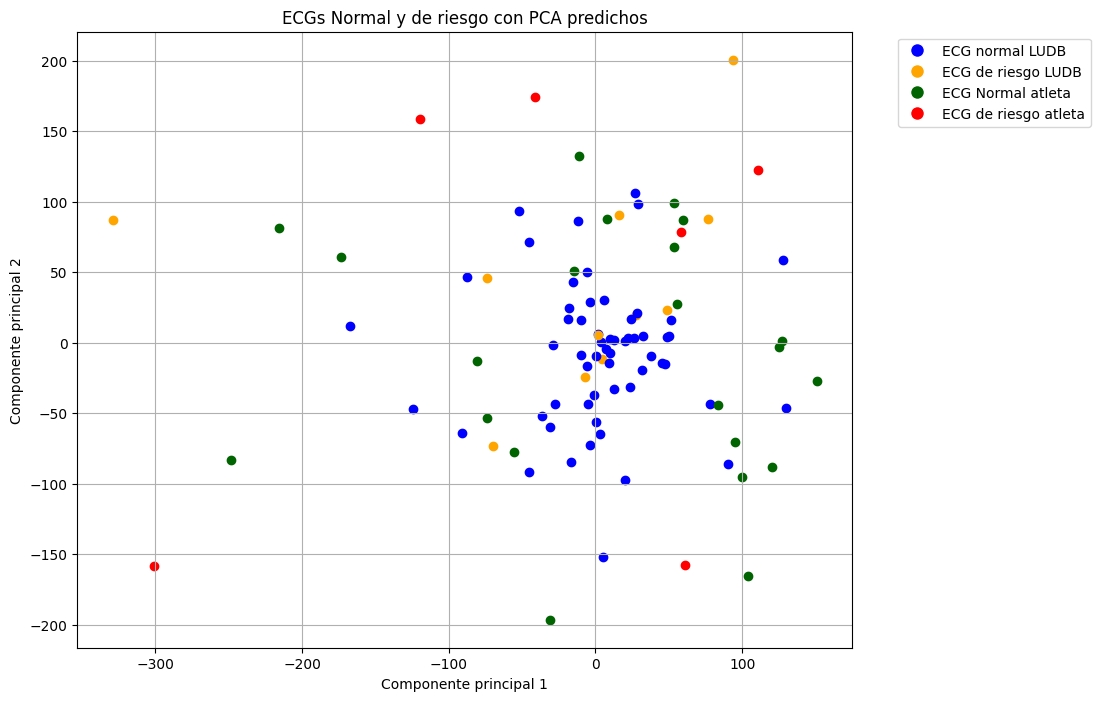
\includegraphics[width=0.5\textwidth]{./graficos/graficoPCAPredicho.png}
    \caption{Gráfico PCA con etiquetas predichas}
\end{figure}

\subsection{Gráfico con etiquetas de modelo y con etiquetas del SL12}
\begin{figure}[H]
    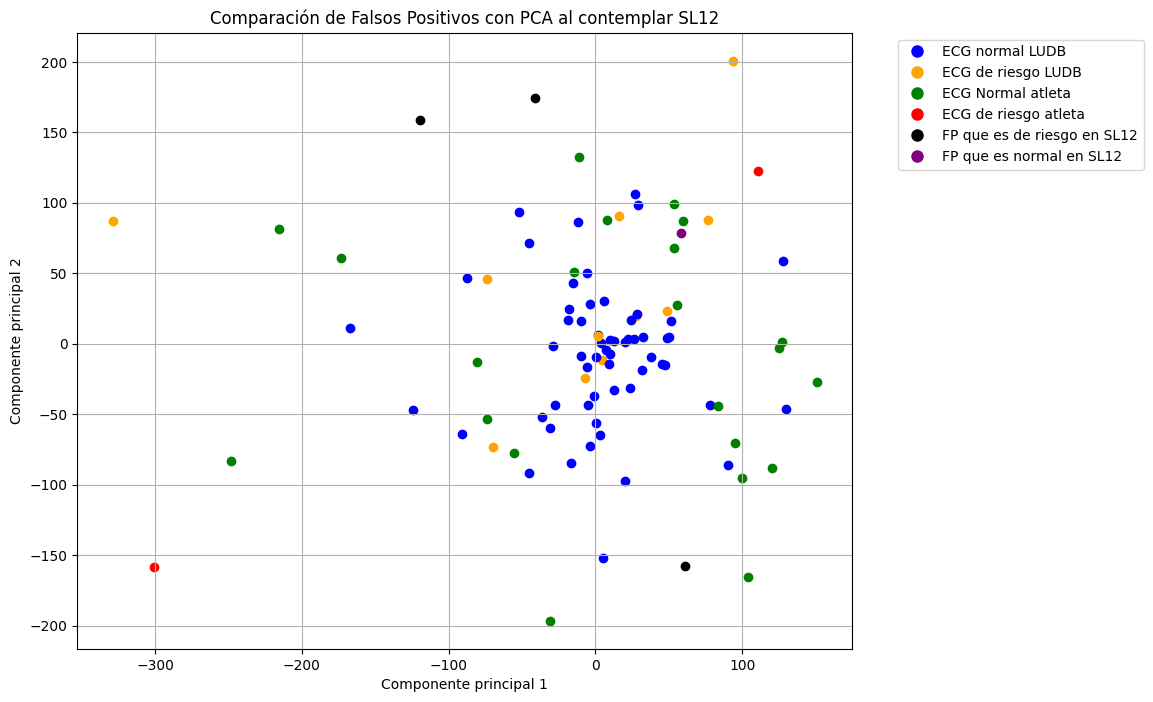
\includegraphics[width=0.5\textwidth]{./graficos/graficoPCAPredichoComparacion.png}
    \caption{Gráfico PCA con etiquetas de SL12 y predicción}
\end{figure}

De los gráficos se puede analizar que los ECG detectados como de riesgo se encuentran 
hacia los bordes del gráfico, separados de los casos normales, estos casos se acercan 
más a ECGs que están clasificados como de riesgo. Sin embargo, según el cardiólogo, 
este corresponde a un ECG normal, lo que nos indica un posible falso positivo.

Para evaluar la veracidad de estos falsos positivos, se comprobarán las etiquetas del
 algoritmo SL12. Para este caso se clasifican como, un FP con riesgo en etiqueta SL12 y un FP normal en SL12. 

Se tiene que los FP que tienen riesgo en la etiqueta SL12, se ubican en los bordes del 
gráfico, ya que estos se encuentran distanciados de la zona en donde se agrupa la gran 
mayoría de los ECG normales. Esto indica que estos casos de falsos positivos si presentan
 una diferencia frente a los casos normales, por lo que detectar estos casos es un acierto, 
 ya que posiblemente se necesite la evaluación de un cardiólogo para descartar un caso de riesgo.
El caso que se consideró de riesgo y si era normal en la etiqueta del SL12 se encuentra 
cercano a los ECGs normales, por lo que se tiene realmente un falso positivo.





\section{Conclusiones}

Al realizar el entrenamiento del modelo KNN con DTW con la BD Lobachevsky University y 
las pruebas con la BD de Atletas Noruegos se obtuvieron resultados aceptables, el aspecto a 
destacar es que se detectaron satisfactoriamente todos los casos de riesgos. Esto es un aspecto 
importante, ya que es crucial no descartar ninguno de estos casos. Sin embargo, se generaron 
algunos falsos positivos, pero esto no es un total error, ya que como se demostró anteriormente, 
al contemplar el diagnóstico del algoritmo SL12, es posible que estos casos también necesitaban 
la evaluación de un cardiólogo para descartar los riesgos. 

Analizando el gráfico PCA, se logró comprobar e identificar que existe un sesgo cuando se tiene 
casos de riesgo, ya que estos se alejan de la zona donde se agrupan los casos normales. 
Además, los casos que fueron identificados como falsos postivos que resultaron de riesgo en 
la etiqueta del algoritmo SL12, se encuentran separados de la zona en donde se agrupan los 
casos normales, representando una división entre los casos normales y los de riesgo. 

El modelo logra buenos resultados, y se entrega un diagnóstico enfocado a deportistas. 
Sin embargo, el algoritmo se vuelve lento al tener muchos datos, una mejora seria optimizar 
la implementacion del DTW para que el algoritmo disgnostique en un menor tiempo.

\begin{thebibliography}{00}
\bibitem{b1} Singstad, B. (2022). Norwegian Endurance Athlete ECG Database (version 1.0.0). PhysioNet. https://doi.org/10.13026/qpjf-gk87.
\bibitem{b2} Kalyakulina, A., Yusipov, I., Moskalenko, V., Nikolskiy, A., Kosonogov, K., Zolotykh, N., \& Ivanchenko, M. (2021). Lobachevsky University Electrocardiography Database (version 1.0.1). PhysioNet. https://doi.org/10.13026/eegm-h675.
\bibitem{b3} Drezner JA, Sharma S, Baggish A, et al. International criteria for electrocardiographic interpretation in athletes: Consensus statement. Br J Sports Med. 2017;51:704-731 
\end{thebibliography}
\end{document}
